\subsection{Hypothesis 1}
\begin{figure}[ht!]
\centering
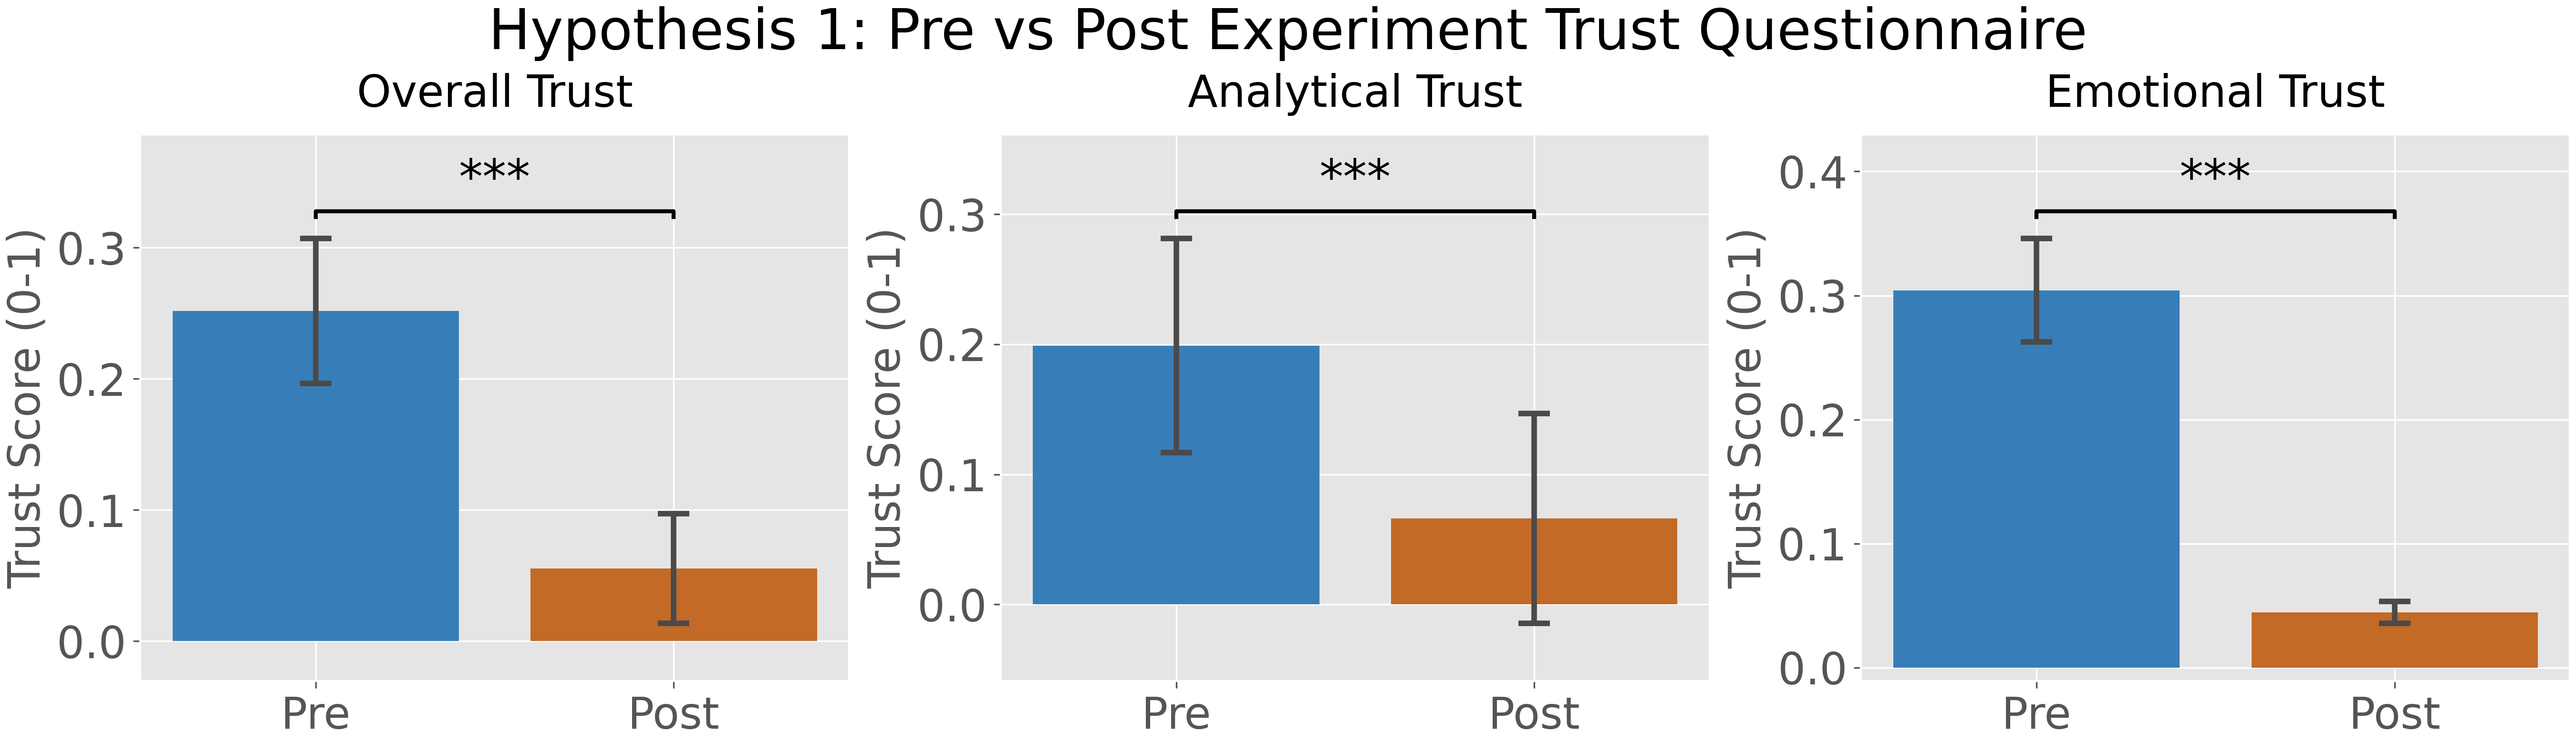
\includegraphics[width=0.85\linewidth]{Figures/hypothesis1.png}
\caption{Visualization for Hypothesis 1.}
\label{fig:hypothesis1}
\end{figure}

To begin our statistical analysis with Hypothesis 1, we perform a comparison of the pre and post experiment questionnaires in terms of overall, analytical alone, and emotional alone self-reported trust. This results in three sub-hypotheses related to this hypothesis that can each be individually tested for statistical significance. 

Hypothesis 1.1 compares the pre-post experiment overall trust, to evaluate the significance in the change in reported trust when combining emotional and analytical definitions. We performed a two-tailed paired-samples t-test ($\alpha=.05$) and a two-sided Wilcoxon signed-rank test on pre-post overall trust scores, which showed $n=504$, $M_{pre}=4.728$, $SD_{pre}=12.319$, $M_{post}=1.062$, $SD_{post}=9.561$, $t(503)=10.395$, $p < .001$, $W=27993.500$, $p_{W} < .001$, $d=-0.463$, $\Delta=-3.667$, sub-hypothesis supported. Hypothesis 1.2 compares the pre-post experiment analytical trust, to evaluate the significance in the change in reported analytical trust. We performed the same two-tailed paired-samples t-test and two-sided Wilcoxon signed-rank test on pre-post analytical trust scores, which showed $n=504$, $M_{pre}=1.990$, $SD_{pre}=9.439$, $M_{post}=0.661$, $SD_{post}=9.238$, $t(503)=4.854$, $p < .001$, $W=35605.500$, $p_{W} < .001$, $d=-0.216$, $\Delta=-1.329$, sub-hypothesis supported. Hypothesis 1.3 compares the pre-post experiment emotional trust, to evaluate the significance in the change in reported emotional trust. We performed the same two-tailed paired-samples t-test and two-sided Wilcoxon signed-rank test on pre-post emotional trust scores, which showed $n=504$, $M_{pre}=2.738$, $SD_{pre}=4.309$, $M_{post}=0.401$, $SD_{post}=0.917$, $t(503)=12.796$, $p < .001$, $W=15999.000$, $p_{W} < .001$, $d=-0.570$, $\Delta=-2.337$, sub-hypothesis supported.

These results demonstrate that there is a significant change in the reported trust when averaging over each condition (Interactive vs. Text), type of trust (Emotional vs. Analytical), and demographic groups (WEIRD vs. NORMAL). This provides the necessary statistical foundation supporting our first hypothesis. Additionally, this overall difference supports the structuring of the following statistical tests used to evaluate the subsequent hypotheses. 

\subsection{Hypothesis 2}
\begin{figure}[ht!]
\centering
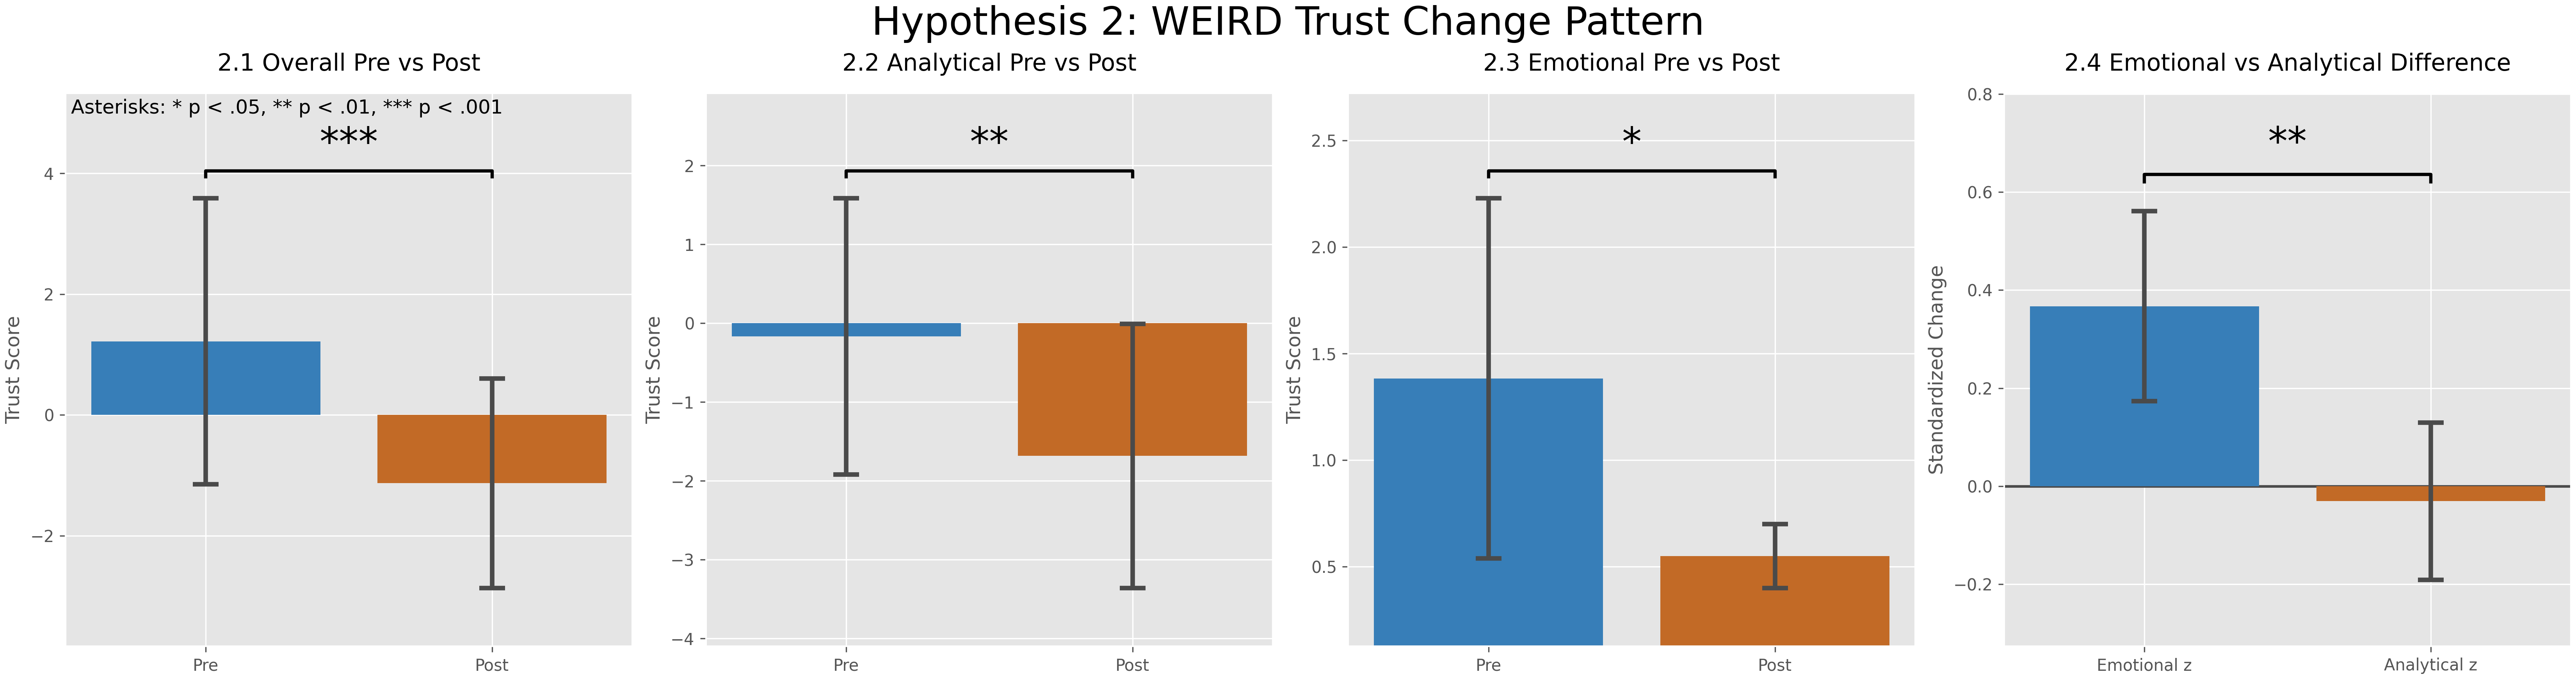
\includegraphics[width=0.85\linewidth]{hypotheses/hypothesis2/hypothesis2.png}
\caption{Visualization for Hypothesis 2.}
\label{fig:hypothesis2}
\end{figure}

For Hypothesis 2, we evaluate WEIRD participants only and test whether overall, analytical, and emotional trust all decrease from pre to post, and whether the standardized emotional-versus-analytical change differs in magnitude. This produces four sub-hypotheses that are each evaluated with inferential statistics.

Hypothesis 2.1 compares pre-post overall trust within WEIRD participants. We performed a two-tailed paired-samples t-test ($\alpha=.05$) and a two-sided Wilcoxon signed-rank test, which showed $n=120$, $M_{pre}=1.217$, $M_{post}=-1.133$, $t(119)=3.440$, $p < .001$, $W=1848.000$, $p_{W} < .001$, $d=-0.314$, $\Delta=-2.350$, sub-hypothesis supported. Hypothesis 2.2 compares pre-post analytical trust within WEIRD participants. We performed the same two-tailed paired-samples t-test and two-sided Wilcoxon signed-rank test, which showed $n=120$, $M_{pre}=-0.167$, $M_{post}=-1.683$, $t(119)=3.014$, $p = .003$, $W=1624.500$, $p_{W} = .003$, $d=-0.275$, $\Delta=-1.517$, sub-hypothesis supported. Hypothesis 2.3 compares pre-post emotional trust within WEIRD participants. We performed the same two-tailed paired-samples t-test and two-sided Wilcoxon signed-rank test, which showed $n=120$, $M_{pre}=1.383$, $M_{post}=0.550$, $t(119)=2.058$, $p = .042$, $W=1936.000$, $p_{W} = .041$, $d=-0.188$, $\Delta=-0.833$, sub-hypothesis supported. Hypothesis 2.4 compares standardized emotional and analytical change within WEIRD participants. We performed a paired comparison using a two-tailed paired-samples t-test and a two-sided Wilcoxon signed-rank test, which showed $n=120$, $M_{em,z}=0.367$, $M_{an,z}=-0.030$, $t(119)=3.301$, $p = .001$, $W=2436.000$, $p_{W} = .002$, $d=0.301$, $\Delta_{z}=0.398$, sub-hypothesis supported.

These results indicate that WEIRD participants show significant decreases across all three trust aggregates and a significant emotional-versus-analytical standardized difference, supporting Hypothesis 2.

\subsection{Hypothesis 3}
\begin{figure}[ht!]
\centering
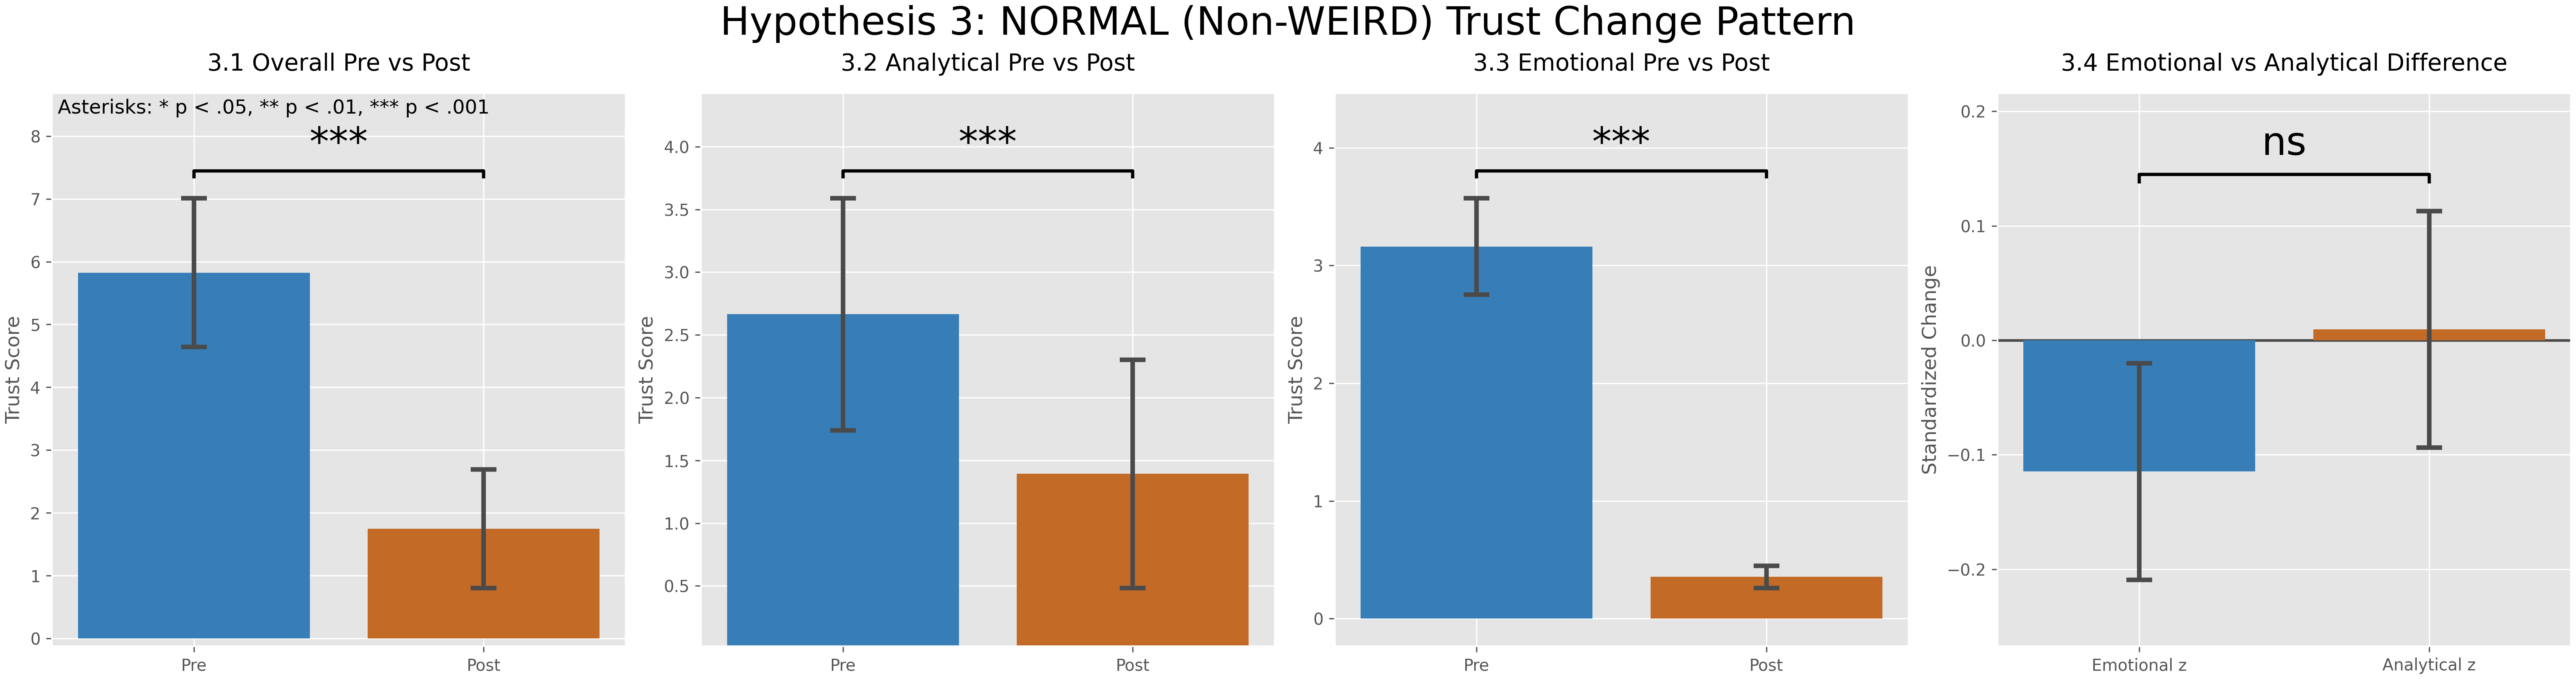
\includegraphics[width=0.85\linewidth]{hypotheses/hypothesis3/hypothesis3.png}
\caption{Visualization for Hypothesis 3.}
\label{fig:hypothesis3}
\end{figure}

For Hypothesis 3, we evaluate NORMAL (non-WEIRD) participants and test whether overall, analytical, and emotional trust decrease from pre to post, while expecting no strong difference between standardized emotional and analytical change.

Hypothesis 3.1 compares pre-post overall trust within NORMAL participants. We performed a two-tailed paired-samples t-test ($\alpha=.05$) and a two-sided Wilcoxon signed-rank test, which showed $n=384$, $M_{pre}=5.826$, $M_{post}=1.747$, $t(383)=9.970$, $p < .001$, $W=15536.500$, $p_{W} < .001$, $d=-0.509$, $\Delta=-4.078$, sub-hypothesis supported. Hypothesis 3.2 compares pre-post analytical trust within NORMAL participants. We performed the same two-tailed paired-samples t-test and two-sided Wilcoxon signed-rank test, which showed $n=384$, $M_{pre}=2.664$, $M_{post}=1.393$, $t(383)=3.928$, $p < .001$, $W=21912.000$, $p_{W} = .002$, $d=-0.200$, $\Delta=-1.271$, sub-hypothesis supported. Hypothesis 3.3 compares pre-post emotional trust within NORMAL participants. We performed the same two-tailed paired-samples t-test and two-sided Wilcoxon signed-rank test, which showed $n=384$, $M_{pre}=3.161$, $M_{post}=0.354$, $t(383)=14.183$, $p < .001$, $W=6354.500$, $p_{W} < .001$, $d=-0.724$, $\Delta=-2.807$, sub-hypothesis supported. Hypothesis 3.4 compares standardized emotional and analytical change within NORMAL participants. We performed a paired comparison using a two-tailed paired-samples t-test and a two-sided Wilcoxon signed-rank test, which showed $n=384$, $M_{em,z}=-0.115$, $M_{an,z}=0.010$, $t(383)=-1.923$, $p = .055$, $W=32037.000$, $p_{W} = .024$, $d=-0.098$, $\Delta_{z}=-0.124$.

These results show strong pre-post trust decreases in NORMAL participants across overall, analytical, and emotional trust. For the emotional-versus-analytical standardized contrast, the t-test is non-significant while Wilcoxon is significant, indicating mixed but small-magnitude evidence relative to the hypothesis expectation.

\subsection{Hypothesis 4}
\begin{figure}[ht!]
\centering
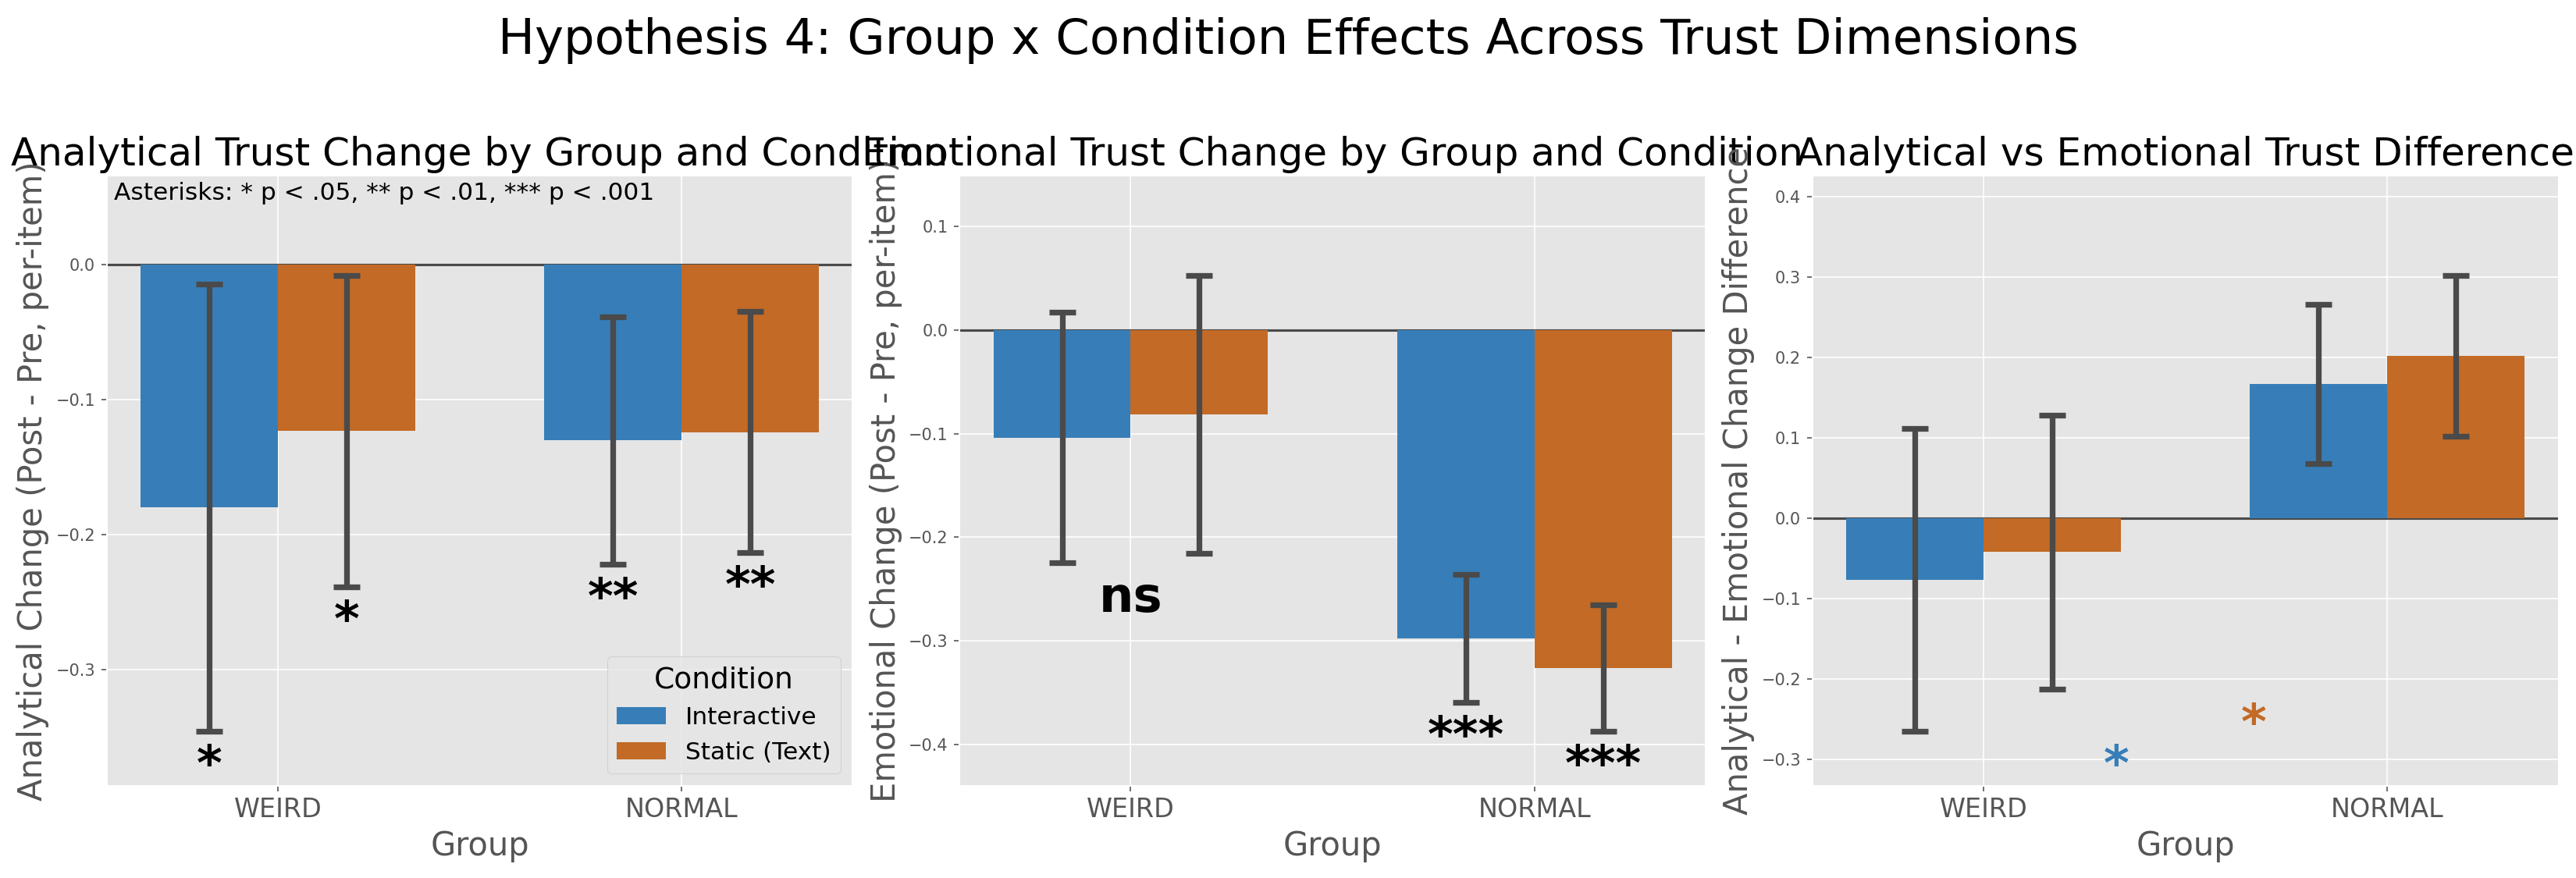
\includegraphics[width=0.85\linewidth]{hypotheses/hypothesis4/hypothesis4.png}
\caption{Visualization for Hypothesis 4.}
\label{fig:hypothesis4}
\end{figure}

For Hypothesis 4, we test Group $\times$ Condition effects across analytical trust change, emotional trust change, and the analytical-versus-emotional difference metric in a three-panel design. All trust-change outcomes are computed as average change scores (Post - Pre).

Hypothesis 4.1 evaluates analytical trust change by Group $\times$ Condition. We performed within-cell pre-post paired-samples t-tests, plus an omnibus four-cell ANOVA and an OLS interaction estimate. Paired results were WEIRD/Interactive: $t(59)=2.17$, $p = .034$, $\Delta M=-0.180$; WEIRD/Static (Text): $t(59)=2.14$, $p = .037$, $\Delta M=-0.123$; NORMAL/Interactive: $t(191)=2.81$, $p = .006$, $\Delta M=-0.130$; NORMAL/Static (Text): $t(191)=2.74$, $p = .007$, $\Delta M=-0.124$. Omnibus ANOVA: $F=0.14$, $p = .938$. Interaction estimate: $b=-0.050$, $t(500)=-0.39$, $p = .696$. Hypothesis 4.2 evaluates emotional trust change by Group $\times$ Condition with the same test structure. Paired results were WEIRD/Interactive: $t(59)=1.71$, $p = .092$, $\Delta M=-0.104$; WEIRD/Static (Text): $t(59)=1.22$, $p = .229$, $\Delta M=-0.081$; NORMAL/Interactive: $t(191)=9.48$, $p < .001$, $\Delta M=-0.297$; NORMAL/Static (Text): $t(191)=10.57$, $p < .001$, $\Delta M=-0.326$. Omnibus ANOVA: $F=7.49$, $p < .001$. Interaction estimate: $b=-0.051$, $t(500)=-0.55$, $p = .585$. Hypothesis 4.3 evaluates analytical-vs-emotional change difference by Group $\times$ Condition. We performed Welch independent-samples tests within each condition, plus an omnibus four-cell ANOVA and an OLS interaction estimate. Condition-level Welch results were Interactive: $t=-2.28$, $p = .025$, $M_{WEIRD}=-0.076$, $M_{NORMAL}=0.167$; Static (Text): $t=-2.46$, $p = .015$, $M_{WEIRD}=-0.042$, $M_{NORMAL}=0.202$. Omnibus ANOVA: $F=3.82$, $p = .010$. Interaction estimate: $b=0.001$, $t(500)=0.01$, $p = .996$.

Overall, Hypothesis 4 shows meaningful main-pattern differences and significant within-condition group differences for the analytical-vs-emotional metric, but no reliable Group $\times$ Condition interaction in the regression interaction terms.

\subsection{Exploratory Qualitative Analysis Results}
\begin{figure}[ht!]
\centering
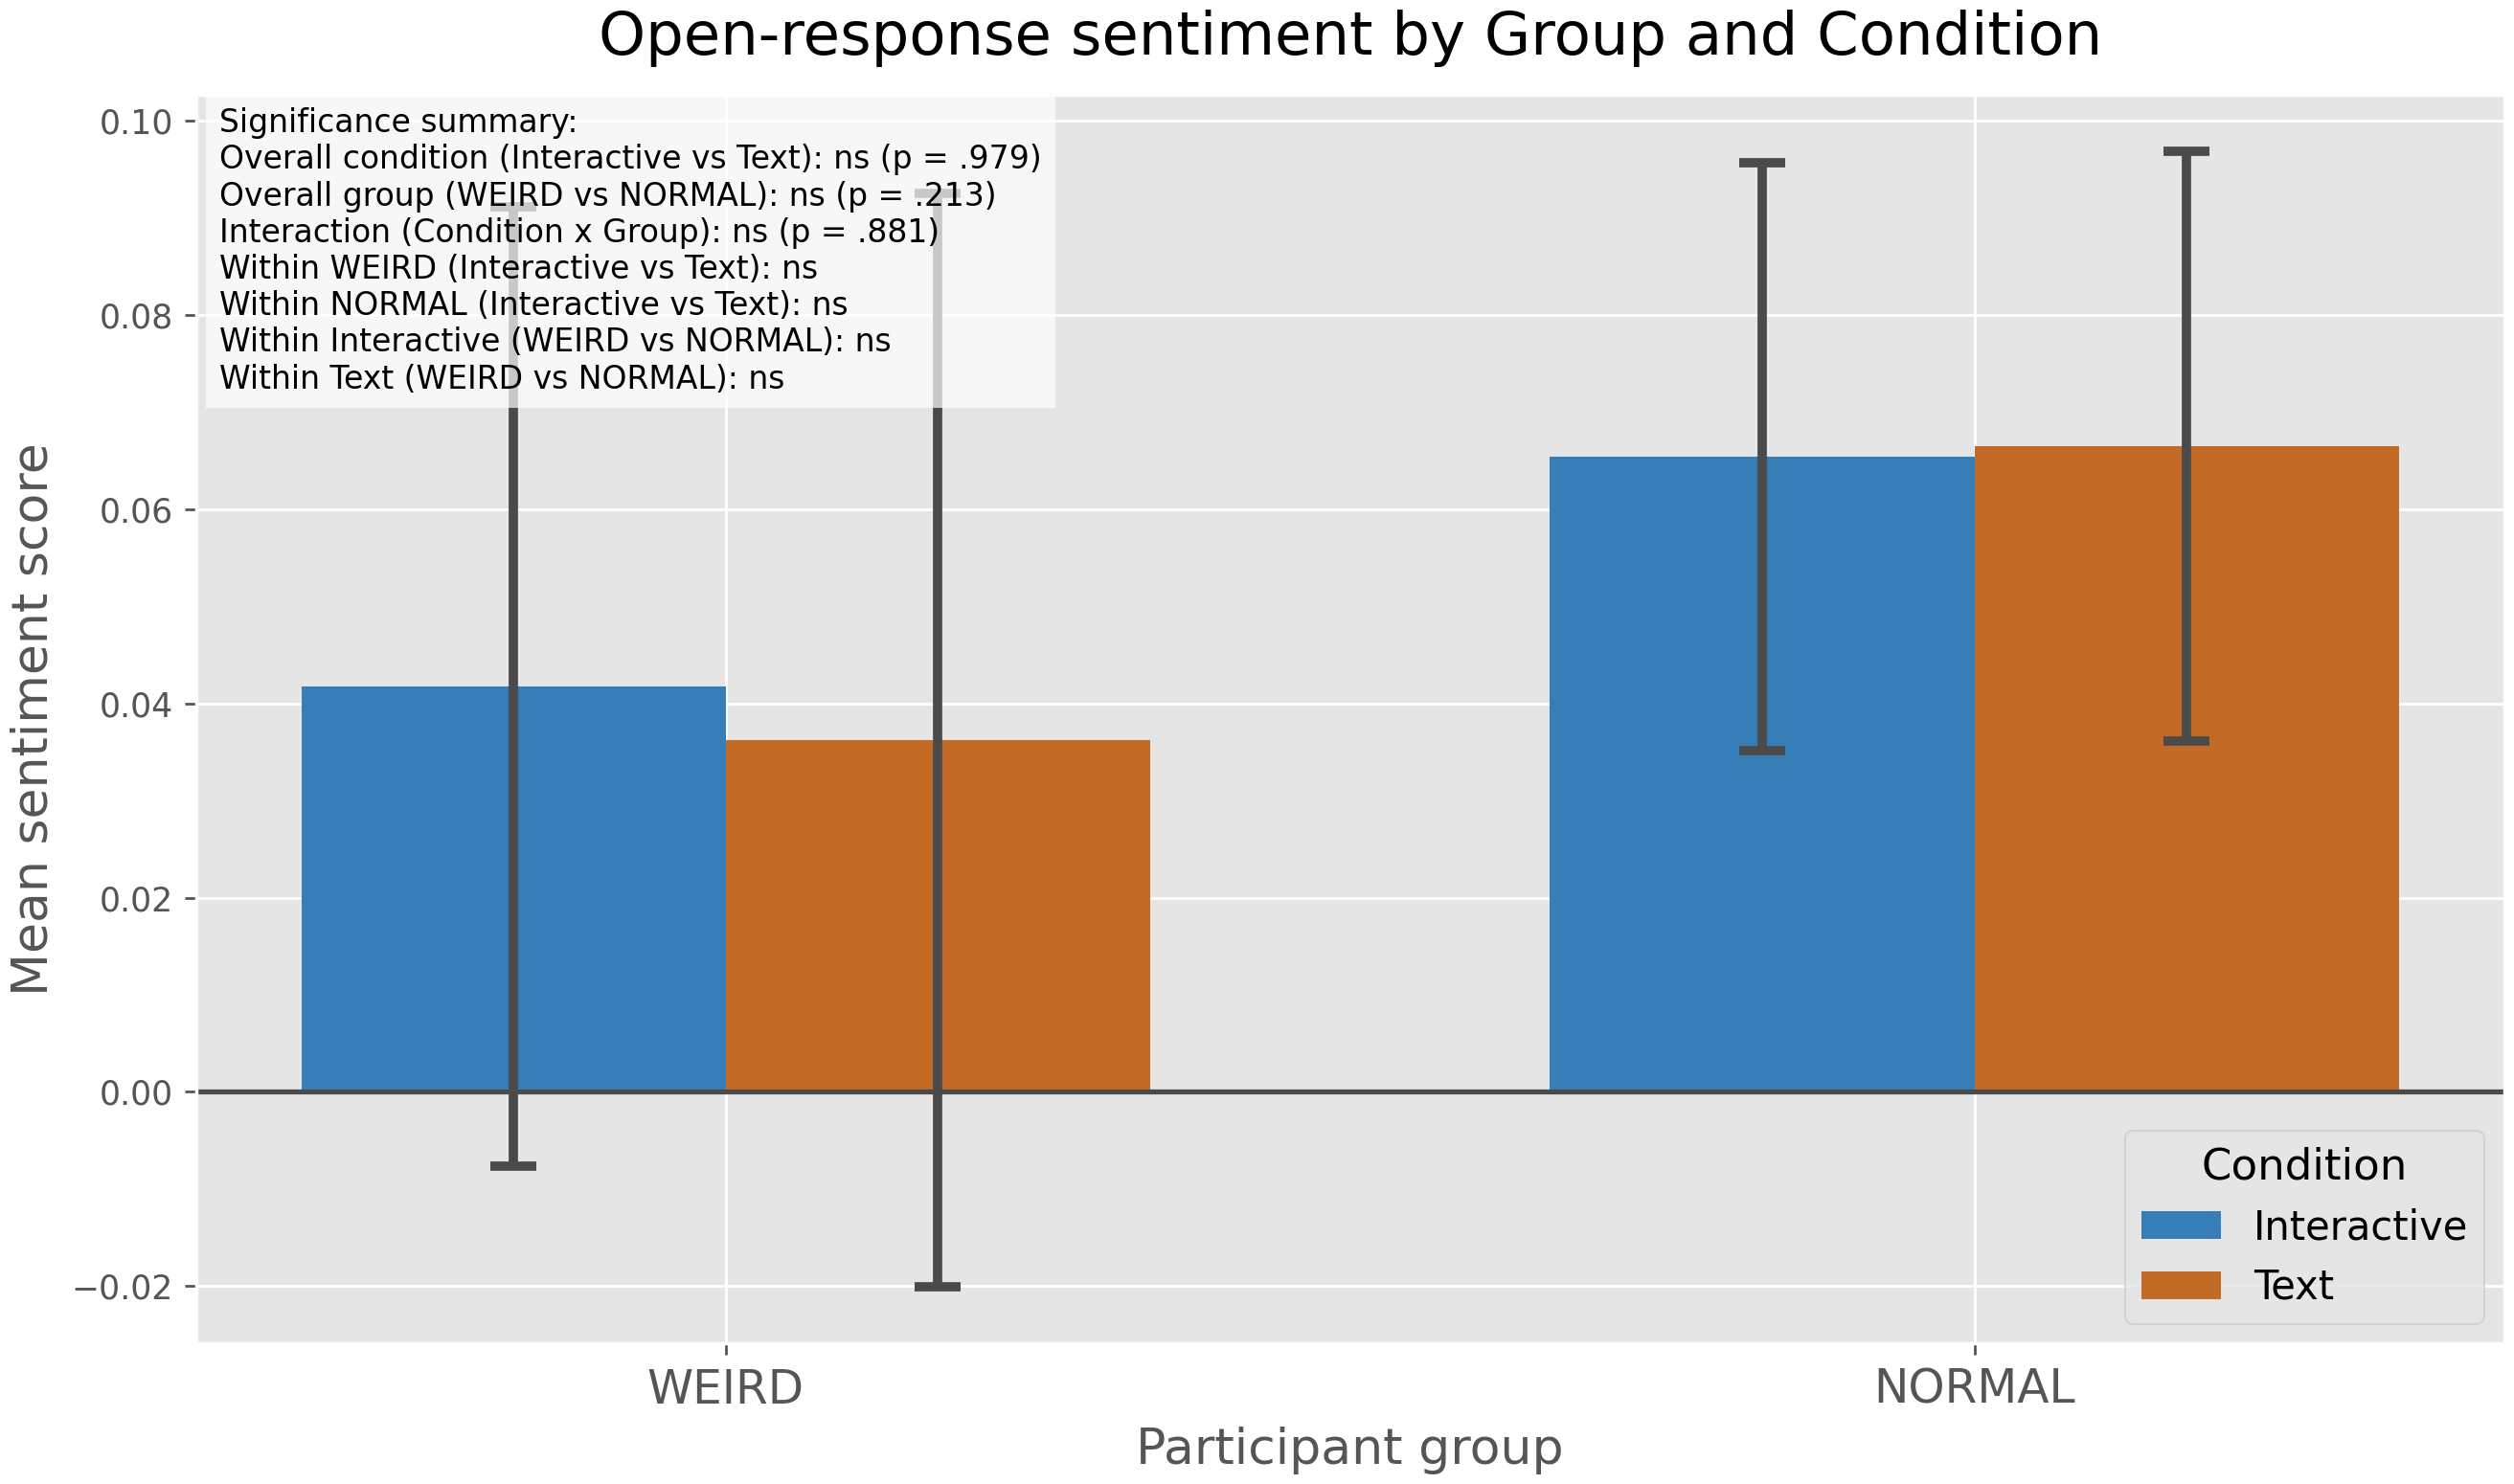
\includegraphics[width=0.9\linewidth]{exploratory_qualitative_analysis/results/sentiment_by_group_condition.png}
\caption{Open-response sentiment by group and condition.}
\label{fig:exploratory_sentiment_group_condition}
\end{figure}

\begin{figure}[ht!]
\centering
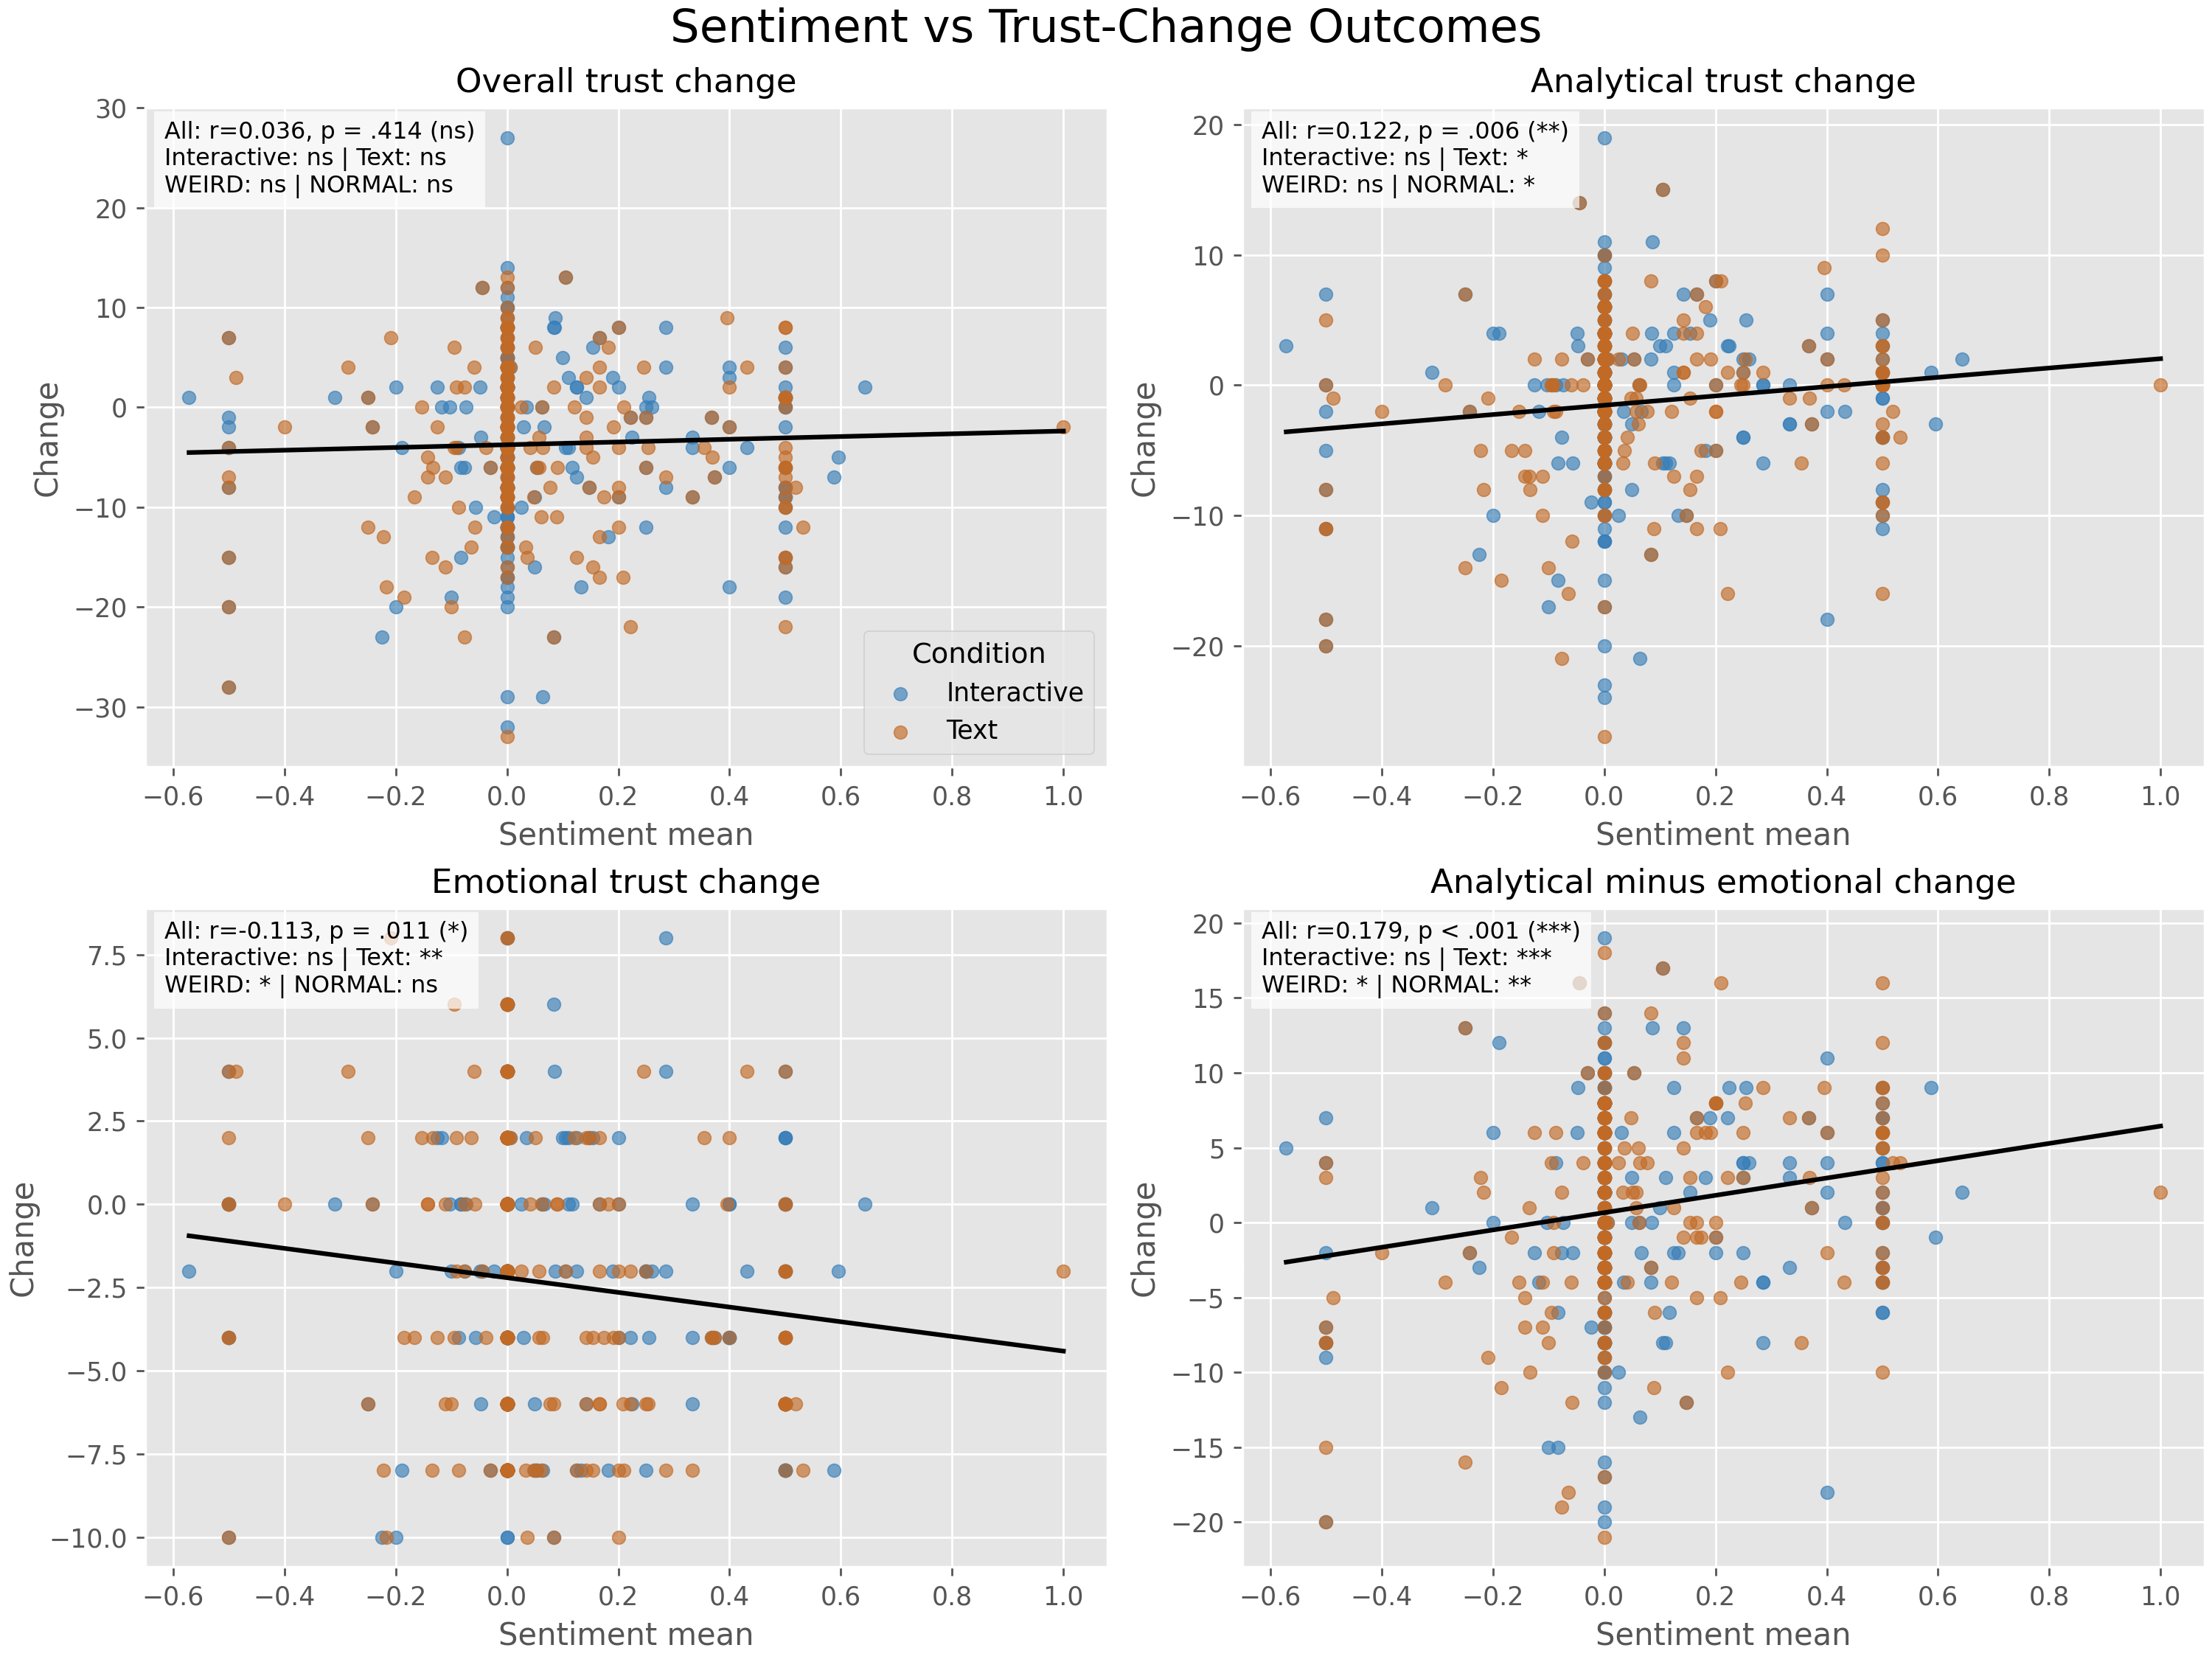
\includegraphics[width=0.92\linewidth]{exploratory_qualitative_analysis/results/sentiment_vs_trust_changes.png}
\caption{Sentiment versus trust-change outcomes.}
\label{fig:exploratory_sentiment_trust_changes}
\end{figure}

To complement the quantitative hypothesis tests, we performed an exploratory qualitative sentiment analysis on open-response text fields (AI Interaction Feeling, AI Definition Feeling, Explanation Comment). We analyzed $n=504$ participants and tested whether sentiment differs by condition and WEIRD/NORMAL grouping and whether sentiment is associated with trust-change outcomes.

For sentiment level differences (group/condition), we performed Welch two-sample tests for condition contrasts and group contrasts and fit an OLS interaction model (Condition $\times$ Group). The overall condition contrast was non-significant ($p = .979$), the overall group contrast was non-significant ($p = .213$), and the interaction term was non-significant ($p = .881$). For sentiment-to-trust associations, we performed Pearson and Spearman correlations in the full sample, with follow-up Pearson tests in condition and group subsets when primary effects were significant. In the primary full-sample tests, overall trust change was non-significant ($p = .414$), analytical trust change was significant ($p = .006$), emotional trust change was significant ($p = .011$), and analytical-minus-emotional trust change was highly significant ($p < .001$). Across the full exploratory module, we ran 28 primary tests (7 significant) and 16 follow-up tests (8 significant).

These exploratory results suggest that sentiment itself did not differ globally by condition or WEIRD grouping, but sentiment variation was meaningfully related to analytical, emotional, and especially analytical-minus-emotional trust change. Because these analyses were exploratory, they should be interpreted as hypothesis-generating evidence for targeted confirmatory models.